% Created 2018-12-13 Thu 11:12
% Intended LaTeX compiler: pdflatex
\documentclass[11pt]{article}
\usepackage[utf8]{inputenc}
\usepackage[T1]{fontenc}
\usepackage{graphicx}
\usepackage{grffile}
\usepackage{longtable}
\usepackage{wrapfig}
\usepackage{rotating}
\usepackage[normalem]{ulem}
\usepackage{amsmath}
\usepackage{textcomp}
\usepackage{amssymb}
\usepackage{capt-of}
\usepackage{hyperref}
\usepackage{minted}
\author{Anoop G R}
\date{\today}
\title{}
\hypersetup{
 pdfauthor={Anoop G R},
 pdftitle={},
 pdfkeywords={},
 pdfsubject={},
 pdfcreator={Emacs 26.1 (Org mode 9.1.9)}, 
 pdflang={English}}
\begin{document}

\tableofcontents


\section{Anoop index:}
\label{sec:orgf90e957}
How Do I Get Started?
Applied Machine Learning Process
Linear Algebra
Statistical Methods
Understand Machine Learning Algorithms
Python Machine Learning (scikit-learn)
Code Algorithm from Scratch (Python)
Introduction to Time Series Forecasting (Python)
XGBoost in Python (Stochastic Gradient Boosting)
Deep Learning (Keras)
Long Short-Term Memory (LSTM)
Deep Learning for Natural Language Processing (NLP)
Deep Learning for Time Series Forecasting


\section{experimental0}
\label{sec:org27defa8}
chrome history suggestions based on a neural network
read to get ideas for projects: \url{https://machinelearningmastery.com/self-study-machine-learning-projects/}
maintain a ml daily blog?
how to get computers to talk to each other using socket programming
use free time with phone to study google maps of Bangalore like guttapalli
buy toothbrush, bigger bulb for room
sabji kitne ki hai app

\section{How Do I Get Started?}
\label{sec:org9e82374}

\subsection{articles-read, worth rereading}
\label{sec:org1294971}
$$ Applied Machine Learning Process
 $$ Intermediate: Python Ecosystem.

\$\$ Step 4: Practice on Datasets. Select datasets to work on and practice the process. 

$$ Practice Machine Learning with Small In-Memory Datasets
 $$ Tour of Real-World Machine Learning Problems
\$\$ Work on Machine Learning Problems That Matter To You

\$\$ Step 5: Build a Portfolio. Gather results and demonstrate your skills. 

$$ Build a Machine Learning Portfolio
 $$ Get Paid To Apply Machine Learning
\$\$ Machine Learning For Money

For more on this top-down approach, see:

$$ The Machine Learning Mastery Method
$$ Machine Learning for Programmers

Many of my students have used this approach to go on and do well in Kaggle competitions and get jobs as Machine Learning Engineers and Data Scientists.

\subsection{notes}
\label{sec:org8314f75}

\subsubsection{intro}
\label{sec:org15fd328}
sckit-learn is higher level than numpy \& scipy
machine learning is a subset of artificial intelligence
artificial learning is a more consistent name for machine learning

\subsubsection{some key word definitions:}
\label{sec:org9442e4b}
Model: A machine learning model can be a mathematical representation
of a real-world process. To generate a machine learning model you will
need to provide training data to a machine learning algorithm to learn
from.

Algorithm: Machine Learning algorithm is the hypothesis set that is
taken at the beginning before the training starts with real-world
data. When we say Linear Regression algorithm, it means a set of
functions that define similar characteristics as defined by Linear
Regression and from those set of functions we will choose one function
that fits the most by the training data.

Training: While training for machine learning, you pass an algorithm
with training data. The learning algorithm finds patterns in the
training data such that the input parameters correspond to the target.
The output of the training process is a machine learning model which
you can then use to make predictions. This process is also called
“learning”.

Regression: Regression techniques are used when the output is
real-valued based on continuous variables. For example, any time
series data. This technique involves fitting a line.

Classification: In classification, you will need to categorize data
into predefined classes. For example, an email can either be ‘spam’ or
‘not spam’.

Target: The target is whatever the output of the input variables. It
could be the individual classes that the input variables maybe mapped
to in case of a classification problem or the output value range in a
regression problem. If the training set is considered then the target
is the training output values that will be considered.

Feature: Features are individual independent variables that act as the
input in your system. Prediction models use features to make
predictions. New features can also be obtained from old features using
a method known as ‘feature engineering’. More simply, you can consider
one column of your data set to be one feature. Sometimes these are
also called attributes. And the number of features are called
dimensions.

Label: Labels are the final output. You can also consider the output
classes to be the labels. When data scientists speak of labeled data,
they mean groups of samples that have been tagged to one or more
labels.

Overfitting: An important consideration in machine learning is how
well the approximation of the target function that has been trained
using training data, generalizes to new data. Generalization works
best if the signal or the sample that is used as the training data has
a high signal to noise ratio. If that is not the case, generalization
would be poor and we will not get good predictions. A model is
overfitting if it fits the training data too well and there is a poor
generalization of new data.

Regularization: Regularization is the method to estimate a preferred
complexity of the machine learning model so that the model generalizes
and the over-fit/under-fit problem is avoided. This is done by adding
a penalty on the different parameters of the model thereby reducing
the freedom of the model.

Parameter and Hyper-Parameter: Parameters are configuration variables
that can be thought to be internal to the model as they can be
estimated from the training data. Algorithms have mechanisms to
optimize parameters. On the other hand, hyperparameters cannot be
estimated from the training data. Hyperparameters of a model are set
and tuned depending on a combination of some heuristics and the
experience and domain knowledge of the data scientist.


\section{\url{https://machinelearningmastery.com/python-machine-learning-mini-course/}}
\label{sec:org237c134}
14Lessons
\subsection{pre requisite \url{https://machinelearningmastery.com/gentle-introduction-to-the-bias-variance-trade-off-in-machine-learning/}}
\label{sec:org021b4c9}
\textbf{Bias Error}
Bias are the simplifying assumptions made by a model to make the target function easier to learn.
Low Bias: Suggests less assumptions about the form of the target function.
High-Bias: Suggests more assumptions about the form of the target function.

Examples of low-bias machine learning algorithms include: Decision Trees, k-Nearest Neighbors and Support Vector Machines.
Examples of high-bias machine learning algorithms include: Linear Regression, Linear Discriminant Analysis and Logistic Regression.

\textbf{Variance Error}
Variance is the amount that the estimate of the target function will change if different training data was used.

Examples of low-variance machine learning algorithms include: Linear Regression, Linear Discriminant Analysis and Logistic Regression.
Examples of high-variance machine learning algorithms include: Decision Trees, k-Nearest Neighbors and Support Vector Machines.

Fig 1. bulls-eye visualise \url{http://scott.fortmann-roe.com/docs/BiasVariance.html}

\subsection{1 - install}
\label{sec:org0dbafa5}
\subsubsection{next time try using this tutorial \url{https://sourabhbajaj.com/mac-setup/Python/numpy.html}}
\label{sec:org43304ab}
\subsubsection{make a new virtualenv}
\label{sec:orgb04bc27}
\begin{minted}[]{shell}
pwd
\end{minted}


Use :session: property to speed up org-babel when possible to use the same session
\begin{minted}[]{bash}
source ~/.bashrc
#mkvirtualenv mlm
workon mlm
which python
\end{minted}

\begin{minted}[]{elisp}
(pyvenv-workon "mlm2")
\end{minted}

\subsubsection{install \url{https://stackoverflow.com/questions/26319762/how-to-install-scipy-stack-with-pip-and-homebrew}}
\label{sec:org9abf3a7}
pip install numpy
brew install gcc
pip install scipy
brew install freetype
pip install matplotlib
pip install nose
pip install pandas
pip install sympy
pip install ipython[all]
brew install pyqt
brew install qt
brew install sip
\#after this edit the 2 scripts
\subsubsection{check if properly isntalled using .\_\(_{\text{version}}\) \_ after import}
\label{sec:org3f444de}

using python snippets inside orgmode \url{https://orgmode.org/worg/org-contrib/babel/languages/ob-doc-python.html}
installed python-mode from package-list-packages for emacs
\begin{minted}[]{common-lisp}
(pyvenv-workon "mlm")
\end{minted}

Fixed some errors using: pip install nose pyparsing python-dateutil pep8
\begin{minted}[]{python}
import sys
import scipy
import numpy
import matplotlib
import pandas
import sklearn

print(f'python: {sys.version}')
print(f'scipy: {scipy.__version__}')
print(f'numpy: {numpy.__version__}')
print(f'matplotlib {matplotlib.__version__}')
print(f'pandas {pandas.__version__}')
print(f'sklearn {sklearn.__version__}')

\end{minted}

\subsection{2 - python, pandas, numpy, mathplotlib veeery basics}
\label{sec:orgb3e4198}

\subsubsection{python, also refer in-y-minutes file for future reference}
\label{sec:orgd4ef033}
\begin{minted}[]{python}
if 1>2:
    print("wtf")
else:
    print("ok")

try:
    # Use "raise" to raise an error
    raise IndexError("This is an index error")
except IndexError as e:
    print("its indexerror")
    pass                 # Pass is just a no-op. Usually you would do recovery here.
except (TypeError, NameError):
    print("its typeerror or nameerror")
    pass                 # Multiple exceptions can be handled together, if required.
else:                    # Optional clause to the try/except block. Must follow all except blocks
    print("All good!")   # Runs only if the code in try raises no exceptions
finally:                 #  Execute under all circumstances
    print("We can clean up resources here")
\end{minted}

\begin{minted}[]{python}
def accepts_variable_number_of_arguments(*args):
    print(type(args))
    print(args)

accepts_variable_number_of_arguments(1,2,3)

def accepts_variable_number_of_keyword_arguments(**kwargs):
    print(type(kwargs))
    print(kwargs)

accepts_variable_number_of_keyword_arguments(name="anoop", work="code")
\end{minted}

\subsubsection{numpy basics}
\label{sec:orgbeb06fc}

\begin{center}
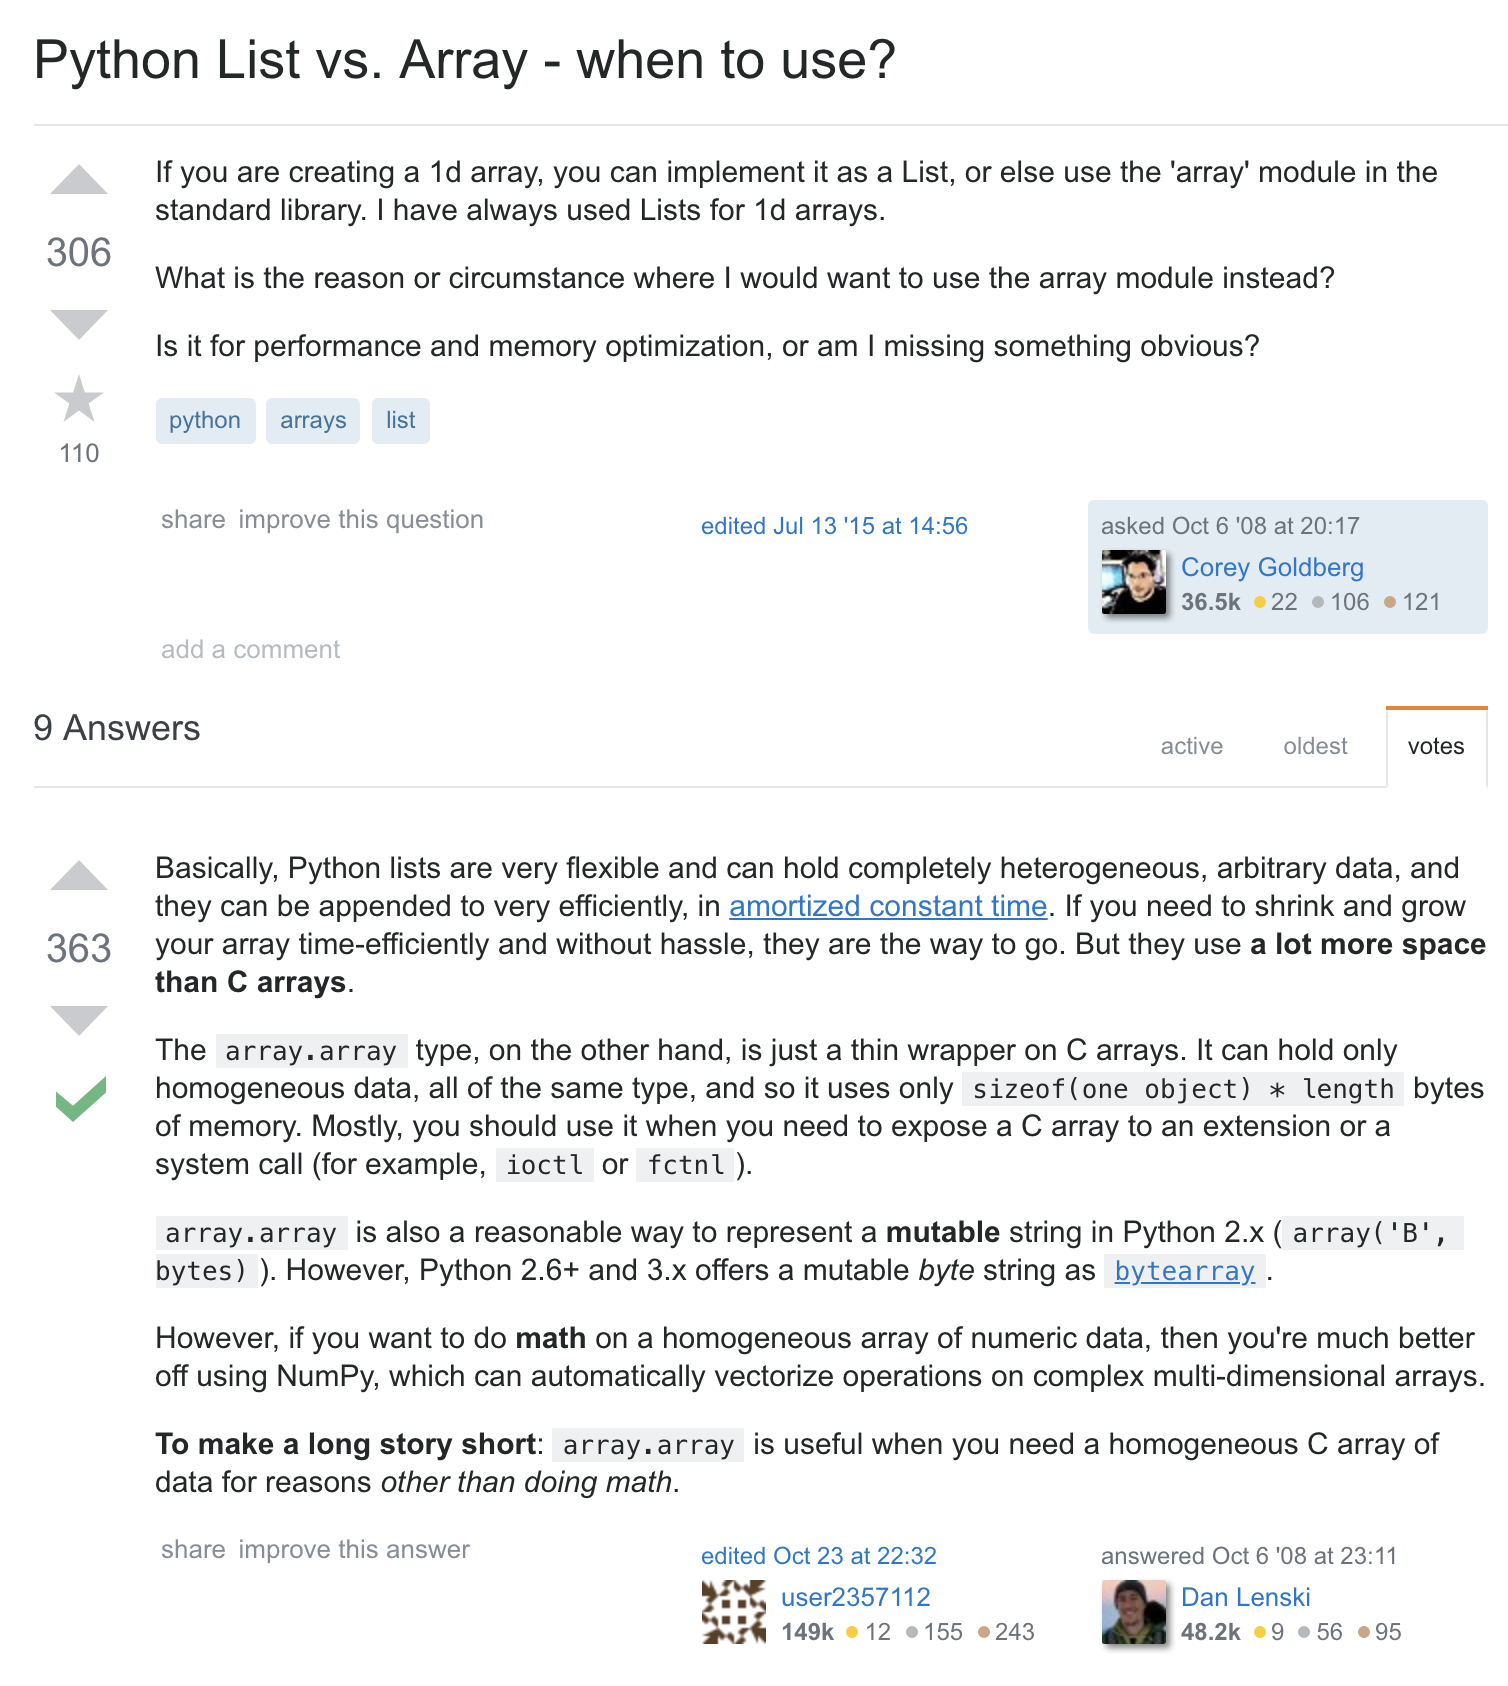
\includegraphics[width=.9\linewidth]{screenshots0/Screenshot 2018-12-11 at 5.16.28 PM.png}
\end{center}

\textbf{numpy official tutorial}
\url{https://docs.scipy.org/doc/numpy-1.15.0/user/quickstart.html}
\begin{minted}[]{python}
  import numpy as np
  a = np.arange(15).reshape(3,5)
  print(a)
  a.shape
  a.ndim
  a.dtype.name
  #dir(a)
  a.size
  type(a)
  b = np.array([6,7,8])
  b
  type(b)

  np.zeros([2,3])
  np.arange(15)
  np.linspace(0,9, 19)

  from numpy import pi
  x = np.linspace(0, 2*pi, 5)
  np.sin(x)
  #2 decimal places
  np.around(np.sin(x), decimals=2)

  A = np.array([[1,2],[3,4]])
  I = np.array([[1,0],[0,1]])
  elementwise = A * I
  matrix_product = A @ I
  print(elementwise, "\n", matrix_product)

  a = np.ones(3, dtype=np.int32)
  b = np.linspace(0, 1, 3)
  c = a + b
  print(a,b,c)
  c.dtype.name
  c*1j
  np.ones(1)
  my_e = np.exp(np.ones(1))
  from numpy import e
  e
  print(e, my_e)
  d = np.exp(c*1j)
  d.dtype
  # exp, sin etc are called numpy universal functions

  # multidimensional array
c = np.array([
    [
	[  0,  1,  2],
	[ 10, 12, 13]
    ],
    [
	[100,101,102],
	[110,112,113]
    ]
])
c.shape
# Visualize0 2,2,3 as you traverse from the topmost bracket to the inner ones
for i in c.flat:
    print(i, end=" // ")
print("\n")
id(c) #id is unique identifier of an object in python


\end{minted}

axis in numpy

\href{screenshots0/Screenshot\%202018-12-11\%20at\%206.06.43\%20PM.png}{file:\textasciitilde{}/ml/flipshope/screenshots0/Screenshot 2018-12-11 at 6.06.43 PM.png}

matplotlib python is not installed as a framework error, solution:
\url{https://stackoverflow.com/questions/34977388/matplotlib-runtimeerror-python-is-not-installed-as-a-framework}

Above is a hacky solution
I need to switch away from virtualenv \& virtualenvwrapper and move to venv entirely
Also, reddit recommends to avoid the pyenv or any wrapper around venv \&\& strongly recommends to use venv directly
venv ships by default with python >= 3.3
\url{https://matplotlib.org/faq/osx\_framework.html}
\url{https://news.ycombinator.com/item?id=18612590}
\url{https://news.ycombinator.com/item?id=18247512}
:) 	
andybak 54 days ago [-]
In case this scares any new users, I've used nothing more than pip and virtualenv for several years with no issues of note.



\begin{minted}[]{python}
import numpy as np
import matplotlib.pyplot as plt
#import matplotlib  
#matplotlib.use('TkAgg')   
#import matplotlib.pyplot as plt 

def mandelbrot( h,w, maxit=20 ):
    """Returns an image of the Mandelbrot fractal of size (h,w)."""
    y,x = np.ogrid[ -1.4:1.4:h*1j, -2:0.8:w*1j ]
    c = x+y*1j
    z = c
    divtime = maxit + np.zeros(z.shape, dtype=int)

    for i in range(maxit):
	z = z**2 + c
	diverge = z*np.conj(z) > 2**2            # who is diverging
	div_now = diverge & (divtime==maxit)  # who is diverging now
	divtime[div_now] = i                  # note when
	z[diverge] = 2                        # avoid diverging too much

    return divtime
plt.imshow(mandelbrot(400,400))
plt.show()
\end{minted}

\begin{minted}[]{python}
import sys
print(sys.path)
\end{minted}

\textbf{real-python tutorial}
\url{https://realpython.com/numpy-array-programming/}

When it comes to computation, there are really three concepts that lend NumPy its power:
Vectorization
Broadcasting
Indexing

\begin{minted}[]{python}
import numpy as np

arr = np.arange(36).reshape(3,4,3)
arr

"""
visualize0:-

00 01 02 03 04 05 06 07 08 09 10 11 
12 13 14 15 16 17 18 19 20 21 22 23 
24 25 26 27 28 29 30 31 32 33 34 35 

00 01 02 
03 04 05 
06 07 08 
09 10 11 

[#3 items
[#4 items
[]
[]
[]
[]
]...
]
"""
a = np.array([2,3,4])
b = 2
b_broadcasted = np.broadcast(a,b)
print(list(b_broadcasted))
# rest of this tutorial seemed a bit advanced, skip for now, come back later

\end{minted}

\textbf{Note} Pandas is a library built on top of NumPy

todo: switch to jupyter notebook instead of emacs: 
\url{https://github.com/millejoh/emacs-ipython-notebook}
\url{http://millejoh.github.io/emacs-ipython-notebook/}
\url{https://www.youtube.com/watch?v=wtVF5cMhBjg}
\url{https://news.ycombinator.com/item?id=9728143}
\url{https://github.com/gregsexton/ob-ipython}

\subsubsection{matplotlib basics}
\label{sec:org33dea43}
matplotlib, is written in pure Python and is heavily dependent on NumPy

Matplotlib is conceptually divided into three parts:
pylab interface (similar to MATLAB) – pylab tutorial, this is the matplotlib.pyplot import
Matplotlib frontend or API – artist tutorial
backends – drawing devices or renderers

Lets learn pyplot
\url{https://matplotlib.org/users/pyplot\_tutorial.html\#pyplot-tutorial}

venv basics to switch from virtualenv

python3 -m venv mlm2
source mlm2/bin/activate

pyvenv-deactivate

\begin{minted}[]{python}
import matplotlib
#matplotlib.use('MacOSX')
import matplotlib.pyplot as plt

plt.plot([0, 1, 4, 9, 16])
#plt.show()

plt.plot([0, 1, 4, 9, 16], 'ro')
#plt.show()

plt.plot([0.5], 'y.')
plt.show()
\end{minted}

\subsubsection{Pandas -basics:}
\label{sec:orgf77a506}
Todo:\url{https://pandas.pydata.org/pandas-docs/stable/dsintro.html\#dsintro}
Todo:Official beginner tutorial: \url{https://pandas.pydata.org/pandas-docs/stable/10min.html}
Todo: Intermediate - Julia Evans - \url{https://jvns.ca/blog/2013/12/22/cooking-with-pandas/}
"take a real dataset or three, play around with it, and learn how to use pandas along the way."


Panda Series \& DataFrames:
\url{https://medium.freecodecamp.org/series-and-dataframe-in-python-a800b098f68}
\begin{minted}[]{python}
#Series and DataFrames
import pandas as pd
x1 = pd.Series([6,3,4,6])
x = pd.Series([6,3,4,6], index=['a','b','c','d'])
x
y = pd.Series(3, index=['a', 'b', 'c', 'd'])
y

#DataFrames
import numpy as np
dates = pd.date_range('20181201', periods = 8)

my_narray = np.random.randn(8,3)
list('ABC')

df = pd.DataFrame(index = dates, data = my_narray, columns = ['A','B','C'])
df_absolute = df.apply(abs)
\end{minted}

So pandas is kinda like an excel sheet0

\begin{minted}[]{python}
import numpy as np

np.arange(4)
ma = np.arange(4).reshape((2,2))

import pandas

p = pandas.DataFrame(ma)

print(ma[1,0])
print(p[1])
print(p[1][0] == ma[1][0])
print(p.shape)


\end{minted}

\subsection{3 - Load csv}
\label{sec:orgfab12d4}
\url{https://realpython.com/python-csv/}
\url{https://github.com/jbrownlee/Datasets}

\textbf{Work with csv using python's csv module}
\begin{minted}[]{python}
import csv

with open('iris.csv') as csv_file:
    """
    for line in csv_file:
	print(line)
	pass
    """
    csv_reader = csv.reader(csv_file)
    for line in csv_reader:
	#print(line)
	pass

my_fieldnames = ("sepal_length", "sepal_width", "petal_length", "petal_width", "class")

with open('iris.csv') as csv_file:
    csv_dict_reader = csv.DictReader(csv_file, fieldnames=my_fieldnames)
    for line in csv_dict_reader:
	#print(line)
	pass

with open('test_writeout.csv', mode='w') as out_file:
    csv_writer = csv.writer(out_file)
    csv_writer.writerow(["row", "1"])
    csv_writer.writerow(["row", "2"])
    #
    csv_dict_writer = csv.DictWriter(out_file, fieldnames = my_fieldnames)
    csv_dict_writer.writeheader()
    csv_dict_writer.writerow({"sepal_length": 1, "sepal_width": 2, "petal_length": 3, "petal_width": 4, "class": 5})


\end{minted}

\textbf{Work with csv using numpy}
\begin{minted}[]{python}
import numpy as np

with open("numpy_loadtxt_input.txt") as input_file:
    """
    for line in input_file:
	print(line)
    """
    my_nparray = np.loadtxt(input_file, delimiter=" ")
    print(my_nparray)
    print(my_nparray.dtype)
\end{minted}

\textbf{Work with csv usign pandas}
\begin{minted}[]{python}
import pandas
df = pandas.read_csv('pandas_read_csv.csv')
print(df)

df2 = pandas.read_csv('pandas_read_csv.csv', parse_dates=['Hire Date'], index_col='Name')
print(df2)

my_col_names = ("Name", "Hired_on", "Salary", "sick_days_remaining")
df3 = pandas.read_csv('pandas_read_csv.csv', header=None, names=my_col_names,
parse_dates=['Hired_on'])
print(df3)

df3.to_csv('pandas_to_csv.csv')
\end{minted}


\subsection{4 - use pandas.DataFrame helper functions to describe data with statistics}
\label{sec:orgcc50410}
\begin{minted}[]{python}
# Scatter Plot Matrix
import matplotlib.pyplot as plt
import pandas

my_col_names = ("num_preg", "plasma_glucose", "blood_pressure", "triceps_skin_thickness", "serum_insulin", "bmi", "diabetes_pedigree", "age", "class")
df = pandas.read_csv("https://raw.githubusercontent.com/jbrownlee/Datasets/master/pima-indians-diabetes.data.csv", header=None, names=my_col_names)
#print(df)

from pandas.plotting import scatter_matrix

scatter_matrix(df)
plt.show()

df.corr()
\end{minted}
\subsection{5 - Basic Data Visualization}
\label{sec:orgfb49c57}
Using pandas and matplotlib together
\begin{minted}[]{python}
# Scatter Plot Matrix
import matplotlib.pyplot as plt
import pandas

my_fieldnames = ("sepal_length", "sepal_width", "petal_length", "petal_width", "class")
data = pandas.read_csv('iris.csv', names=my_fieldnames)
#print(data)

se = data.loc[data["class"] == "Iris-setosa"]
ve = data.loc[data["class"] == "Iris-versicolor"]
vi = data.loc[data["class"] == "Iris-virginica"]

#se.hist()
#ve.hist()
#vi.hist()

se.plot(kind="box")

from pandas.plotting import scatter_matrix
#scatter_matrix(se)

plt.savefig("img/lesson5.png")
return "img/lesson5.png"
\end{minted}


\subsection{6 - Preprocessing data}
\label{sec:org26d3593}

Standardize numerical data (e.g. mean of 0 and standard deviation of 1) using the scale and center options.

Simple example:
\begin{minted}[]{python}
import numpy
narray = numpy.arange(0,4).reshape(2,2)

import pandas
df = pandas.DataFrame(narray, columns=("c1", "c2"))

from sklearn.preprocessing import StandardScaler
scaler = StandardScaler()
scaler.fit(df) #calculates and store mean & standard-deviation for each column

print(scaler.transform(df))
type(scaler.transform(df))
df_standardized = pandas.DataFrame(scaler.transform(df))
\end{minted}

Complex example:
\begin{minted}[]{python}
import matplotlib.pyplot as plt
import pandas

#df is my short for DataFrame
my_col_names = ("num_preg", "plasma_glucose", "blood_pressure", "triceps_skin_thickness", "serum_insulin", "bmi", "diabetes_pedigree", "age", "class")
df = pandas.read_csv("https://raw.githubusercontent.com/jbrownlee/Datasets/master/pima-indians-diabetes.data.csv", header=None, names=my_col_names)
#print(df)

import numpy
array = df.values

X = array[:, :-1]
Y = array[:, -1:]

from sklearn.preprocessing import StandardScaler
scaler = StandardScaler().fit(X)
X_standardized = scaler.transform(X)

#printout
numpy.set_printoptions(precision=2)
print(X_standardized)

df_standardized = pandas.DataFrame(X_standardized)
df_standardized.describe() #you can see that mean=0, sdev=1 for each column

\end{minted}


\subsubsection{skip for now, come back later}
\label{sec:org57b2bb5}
Normalize numerical data (e.g. to a range of 0-1) using the range option.
Explore more advanced feature engineering such as Binarizing.

\subsection{7 - Resampling}
\label{sec:org3763536}
statistical methods called resampling methods are used to split your training
dataset up into subsets, some are used to train the model and others
are held back and used to estimate the accuracy of the model on
unseen data.

\subsubsection{Google Developers intro to ml}
\label{sec:org3cebe2c}
complete google developers course, its a pre-requisite for this lesson as per me

\begin{enumerate}
\item 1 hello apple or orange using decision tree
\label{sec:orgf508d50}
\begin{minted}[]{python}
from sklearn import tree
features_original = [[140, "smooth"], [130, "smooth"], [150, "bumpy"], [170, "bumpy"]] #weight, texture of fruit
labels_original = ["apple", "apple", "orange", "orange"]

#smooth=1 // bumpy=0
#orange=1 // apple=0
features = [[140, 1], [130, 1], [150, 0], [170, 0]] #weight, texture of fruit
labels = [0, 0, 1, 1]

#train a classifier: 
clf = tree.DecisionTreeClassifier() #instantiate an empty box of rules
clf = clf.fit(features, labels) #learning algorithm fills the above box with rules

#print(clf.predict([[150,0]]))
print(clf.predict([[200,0]]))
\end{minted}


\item 2 Decision Tree visualization
\label{sec:org2d0386a}

\begin{minted}[]{python}
from sklearn.datasets import load_iris
from sklearn import tree
iris = load_iris()
print(dir(iris))

print(iris.feature_names) #in this example data_names is more suitable
print(iris.data[0])

print(iris.target_names)
print(iris.target)

#Resampling:
test_ids = [0,50,100]

import numpy as np

#training data
train_target = np.delete(iris.target, test_ids)
train_data = np.delete(iris.data, test_ids, axis=0)

#testing data
test_target = iris.target[test_ids]
test_data = iris.data[test_ids]

clf = tree.DecisionTreeClassifier()
clf.fit(train_data, train_target)

predicted_target = clf.predict(test_data)
print(f"Reality: {test_data} features is {test_target}")
print(f"Prediction: {test_data} has been predicted as {predicted_target}")

#Visualize: https://medium.com/@rnbrown/creating-and-visualizing-decision-trees-with-python-f8e8fa394176
from sklearn.externals.six import StringIO  
from sklearn.tree import export_graphviz
import pydotplus

dot_data = StringIO() #StringIO() behaves like a file
export_graphviz(clf, out_file=dot_data, feature_names=iris.feature_names, class_names=iris.target_names)
graph = pydotplus.graph_from_dot_data(dot_data.getvalue())  
graph.write_png("img/iris.png")
return "img/iris.png"
\end{minted}
\end{enumerate}
\end{document}
